\documentclass{article}
\usepackage[left=3cm, right=3cm, top=3cm, bottom=3cm]{geometry}
\usepackage{amsmath}
\usepackage{amsfonts}
\usepackage{hyperref}
\usepackage[backend=biber, style=ieee]{biblatex} 
\usepackage{graphicx}
\addbibresource{multielo.bib}
\hypersetup{colorlinks=true,linkcolor=blue,urlcolor=blue}
\title{Multiplayer generalizations of Elo rating system}
\date{\today}
\author{Brent Kerby}
\begin{document}
	\maketitle
	\begin{abstract}
		This is an expository note on generalizations of the Elo rating system to games with any number of players. This
		includes a discussion of pairwise Elo rating, the Plackett-Luce model, Thurstonian models, and TrueSkill.
		An application to Super Metroid Map Randomizer races on the \texttt{racetime.gg} platform is explored as a motivating example. 
	\end{abstract}
	\section{Introduction}
	
	On the \href{https://racetime.gg}{racetime.gg} platform, players compete to finish video games as quickly as possible,
	most often using randomizers to generate a fresh variation of the game in each race. There is no gameplay interaction
	between the players, but all participants share the same randomized instance of the game and try to see who can finish first.
	Currently the platform uses TrueSkill to rank players within each game category. The rankings are visible on a public leaderboard,
	and players can see how many points they gained or lost after each race. 
	
	Some behaviors of the TrueSkill rating system can be surprising and unintuitive to players, and the main purpose of
	this note is to explore these issues and consider possible solutions or alternatives. We consider the application
	to \texttt{racetime.gg} as a motivating example, with a focus on the Super Metroid Map Randomizer in particular. 
	However, the discussion is likely also relevant to other environments using TrueSkill or similar rating systems.
	
	\section{TrueSkill}
	
	TrueSkill is a rating system developed by Microsoft, commonly used for matchmaking in online games. It uses Bayesian inference to
	model a player skill using two numbers, a mean $\mu$ and standard deviation $\sigma$; together these represent a Gaussian prior,
	with $\mu$ representing the expected value of the player's skill, and $\sigma$ representing the standard deviation.
	In simple terms, $\mu$ is the model's best estimate of the player's skill, while $\sigma$ is a measure of the amount of uncertainty in that estimate.
	A full description of how TrueSkill is out of scope of this note as it is quite complex; this information can be found in the 
	TrueSkill paper \cite{herbrich2006trueskill}.
	
	On \texttt{racetime.gg} the following unintuitive behaviors in the rating system have been observed:
	\begin{itemize}
		\item When a game category is first opened, player ratings swing up and down wildly.
		\item A player who finishes last place (or quits before finishing) may still be awarded a gain in points. This happens commonly with new players, often with a large amount of points.
		\item More rarely, a player who finishes first may lose points.
		\item Over time the ratings stagnate: after playing many games, even if a lower-rated player has a big win against top-rated players, they might not earn many points.
	\end{itemize}
	
	We can visualize some of these behaviors by looking at the trajectories of
	player ratings for Super Metroid Map Rando, showing the ratings of the 15 most active players in the first season (Figure \ref{fig:s1_real_scores}):
	\begin{figure}
	\centering
	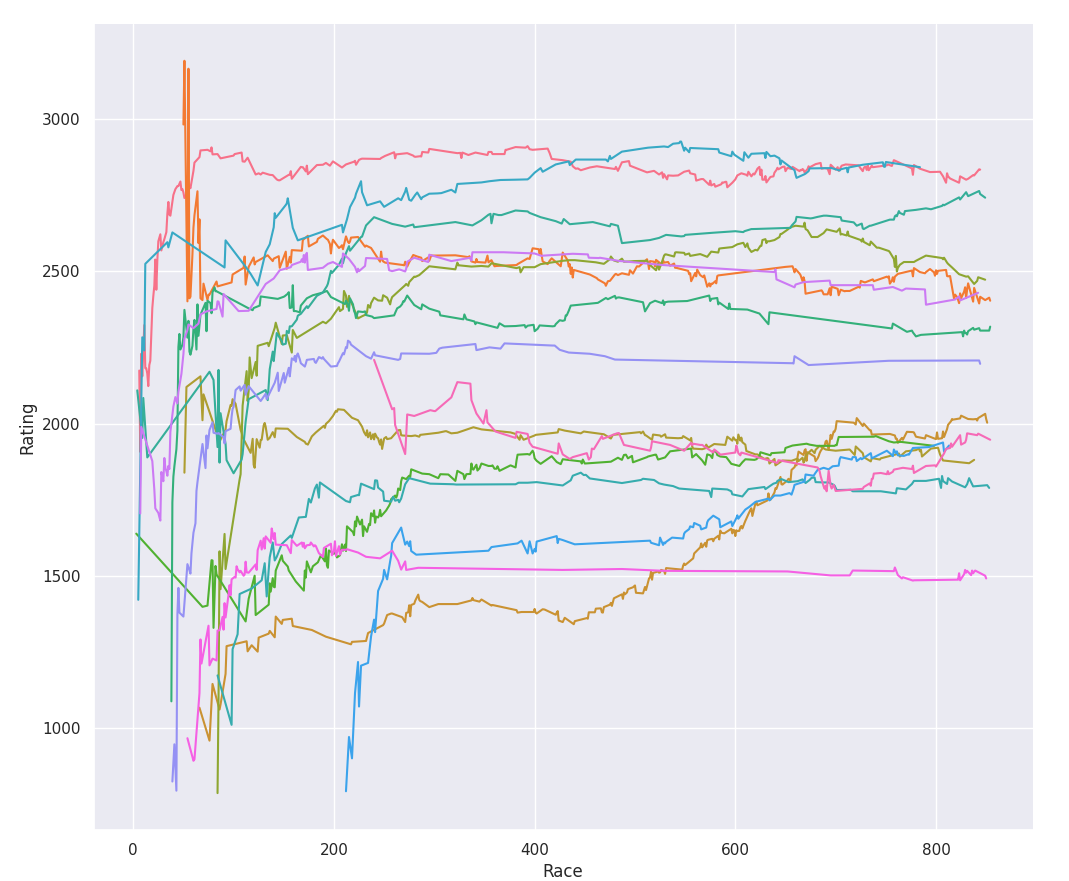
\includegraphics[width=0.75\linewidth]{figures/s1_real_scores.png}
	\caption{Super Metroid Map Rando season 1: recorded scores}
	\label{fig:s1_real_scores}
	\end{figure}
	We can also reproduce these results by replaying the races outcomes offline and simulating the rating updates. This gives similar results (see Figure \ref{fig:s1_trueskill_default}), with some deviations being expected because 1) a few user accounts have since been deleted and their data is no longer available, 2) races may sometimes be recorded in a different order from when they were played.
	\begin{figure}
	\centering
	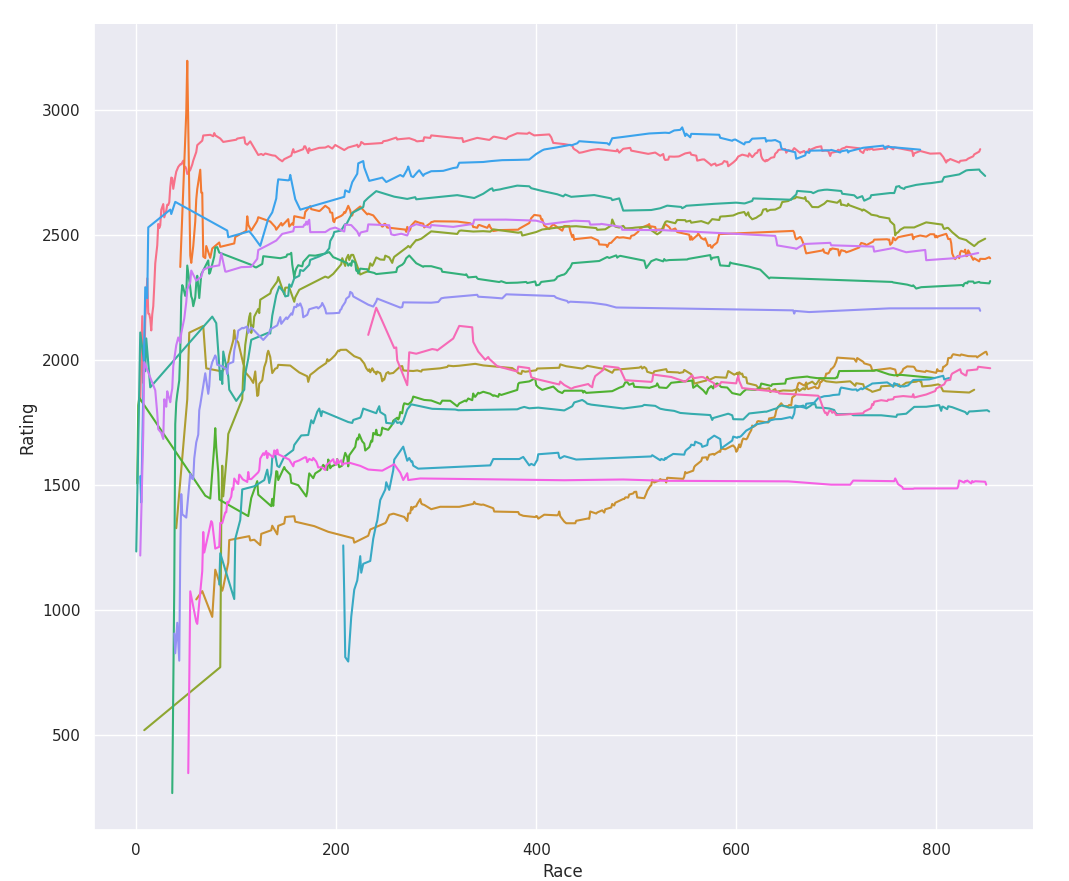
\includegraphics[width=0.75\linewidth]{figures/s1_trueskill_default.png}
	\caption{Super Metroid Map Rando season 1: TrueSkill ratings ($\mu - 2\sigma$), default settings}
	\label{fig:s1_trueskill_default}
	\end{figure}

	The initial volatility and later stagnation of TrueSkill ratings can be explained by the way that the model uses uncertainty parameters $\sigma$. Initially players are assigned a large uncertainty value, at which point a single race result can have a large impact in shifting their rating. As a player participates in races, the uncertainty $\sigma$ decreases over time (see Figure \ref{fig:s1_trueskill_sigma}), resulting in smaller shifts to their rating per race. From a player's perspective, this can be confusing: two players with similar rating could achieve similar results in a race and yet be awarded a very different amount of points. The fact that uncertainty parameters are not visible makes this kind of confusion unavoidable; but even if they were visible, they would probably be challenging for players to interpret.
	\begin{figure}
	\centering
	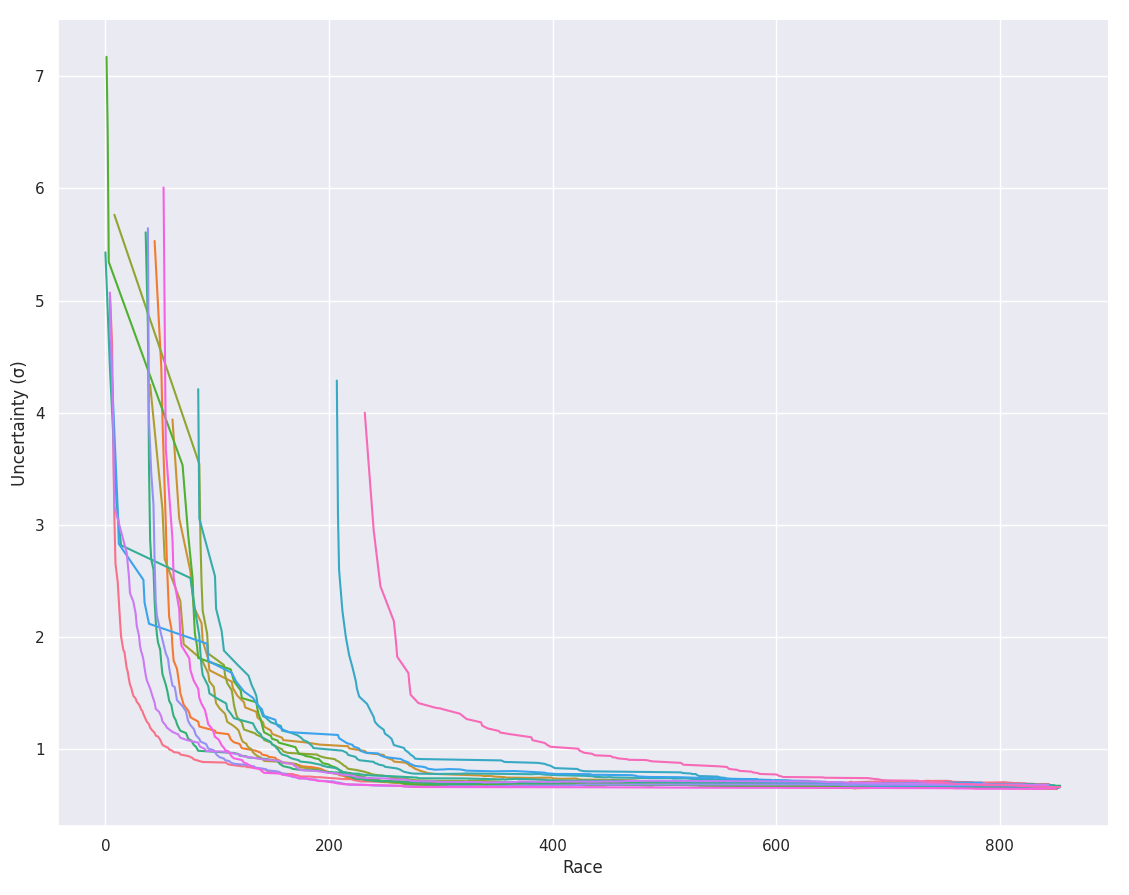
\includegraphics[width=0.75\linewidth]{figures/s1_trueskill_sigma.png}
	\caption{Super Metroid Map Rando season 1: TrueSkill uncertainty values ($\sigma$), default settings}
	\label{fig:s1_trueskill_sigma}
	\end{figure}
	
	It is a recommended common practice to use a lower confidence limit $\mu - 2\sigma$ as the publicly-visible player score used in leaderboard ranking, and \texttt{racetime.gg} uses this. This reduces the possibility of a new, lower-skilled player randomly jumping to the top of the leaderboard. However, this is one potential reason why it could be possible to gain points after getting last place: in this case, the losing player's $\mu$ may decrease, but their $\sigma$ may also decrease enough for the confidence limit $\mu - 2\sigma$ to overall have an increase.
	
	One of the design goals of TrueSkill is to place players as quickly as possible into their correct skill range, to facilitate competitive games when used for matchmaking. From the standpoint of matchmaking, the initial wild swings in a player's rating are not necessarily a problem; exploring matches in which competitors have a wide range of skills can help the system more quickly gain the information it needs to place the player. However, in the context of \texttt{racetime.gg}, matchmaking is not a function that the system provides: in general there is no need for matchmaking here since any number of players can join a race (and though it is possible for tournaments matches to be played on \texttt{racetime.gg}, in this case the matches are defined externally). In this scenario, it might be better if the rating system could behave in a more stable, predictable way, even if it may come with a cost to the speed at which players are initially placed.
	
	\section{Single-parameter rating models}
	The complex and sometimes undesirable behavior that we see with TrueSkill suggests it may be worthwhile to consider simpler systems, ones that use only a single rating parameter per player to model their skill, doing away with the uncertainty parameters used by TrueSkill. For convenience we refer to these as ``single-parameter models", though more precisely they have one parameter per player. We will begin by reviewing the mathematical underpinnings of these systems.
	Readers who are not interested in the mathematical details could skip ahead to section~\ref{sec:convergence}.  
	
	\subsection{Two-player Elo}
	We begin by reviewing the classical 2-player Elo rating system, variations of which are used in chess ratings since the 1960s. We present this system in a form that will generalize to more players. For simplicity, we assume that the game has a simple outcome in which one of the two players wins and the other loses, with no draw being possible. We focus on the ``online" scenario, in which rating updates are applied immediately after each game. The same ideas can be adapted to other scenarios, where rating updates are applied in batches or offline.
	
	\subsubsection{Exponential version}
	During a game, we model the performance of the two players as independent exponential random variables $X_1$ and $X_2$. Writing $\mu_1 = E(X_1)$ and $\mu_2 = E(X_2)$ for the mean performance of player 1 and player 2, the probability density functions of $X_1$ and $X_2$ can be written
	$$f_i(x) = \frac1{\mu_i}e^{-x/\mu_i},\quad i=1, 2$$
	The corresponding cumulative distribution functions are
	$$F_i(x) = P(X_i < x) = 1 - e^{-x/\mu_i},\quad i=1, 2$$
	
	The outcome of the game is modeled as a win for player 1 if $X_1 > X_2$ and a win for player 2 if $X_2 > X_1$. The random variables $X_1$ and $X_2$ are latent: only their order is observable, not their actual values. The mean values $\mu_1$ and $\mu_2$ represent the underlying skill level of the players. Further, write $\mu_i = e^{\rho_i}$ to parametrize player skill on an exponential scale with underlying parameter $\rho_i$. This ensures that any real number $\rho_i$ is associated to a valid, positive skill level $\mu_i$. 
	
	Player ratings $r_i$ will be estimates of the underlying parameters $\rho_i$. The rule for updating player ratings $r_i$ can be defined as a gradient-ascent step in a process of maximizing the log-likelihood of the observed outcome. For example, if player 2 wins, the log-likelihood gradient is defined as
	$$g_i = \left(\frac{\partial}{\partial \rho_i} \log P(X_1 < X_2)\right) \bigg|_{\rho_1=r_1,\ \rho_2=r_2}$$
	The update rule is then defined as
	$$r_i' = r_i + \eta g_i$$
	where $\eta$ is the learning rate (i.e. step size), $r_i$ is the rating of player $i$ before the current game, and $r_i'$ is the updated rating of player $i$ after the current game.
	
	Writing $\lambda_i = 1 / \mu_i$, the probability $P(X_1 < X_2)$ can be computed as
	\begin{align*}
	P(X_1 < X_2) &= \int_0^{\infty} \int_0^{x_2} f_1(x_1) f_2(x_2) dx_1\ dx_2 \\
	&= \int_0^{\infty} f_2(x_2) \int_0^{x_2} f_1(x_1) dx_1\ dx_2 \\
	&= \int_0^{\infty} \frac1{\mu_2}e^{-x_2/\mu_2} \int_0^{x_2} \frac1{\mu_1}e^{-x_1/\mu_1} dx_1\ dx_2 \\
	&= \int_0^{\infty} \lambda_2 e^{-\lambda_2 x_2} \int_0^{x_2} \lambda_1 e^{-\lambda_1 x_1} dx_1\ dx_2 \\
	&= \int_0^{\infty} \lambda_2 e^{-\lambda_2 x_2} (1 - e^{-\lambda_1 x_2})\ dx_2 \\
	&= 1 - \frac{\lambda_2}{\lambda_1 + \lambda_2} \\
	&= \frac{\lambda_1}{\lambda_1 + \lambda_2} \\
	&= \frac{\mu_2}{\mu_1 + \mu_2} \\
	&= \frac{e^{\rho_2}}{e^{\rho_1} + e^{\rho_2}}
	\end{align*}
	
	We can then compute
	\begin{align*}
	\frac{\partial}{\partial \rho_1} \log P(X_1 < X_2)
	&= \frac{\partial}{\partial \rho_1} \log \left(\frac{e^{\rho_2}}{e^{\rho_1} + e^{\rho_2}}\right) \\
	&= \frac{\partial}{\partial \rho_1} (\rho_2 - \log (e^{\rho_1} + e^{\rho_2})) \\
	&= -\frac{e^{\rho_1}}{e^{\rho_1} + e^{\rho_2}} \\
	&= -\frac{\mu_1}{\mu_1 + \mu_2} \\
	\end{align*}
	and
	\begin{align*}
	\frac{\partial}{\partial \rho_2} \log P(X_1 < X_2)
	&= \frac{\partial}{\partial \rho_2} (\rho_2 - \log (e^{\rho_1} + e^{\rho_2})) \\
	&= 1 - \frac{e^{\rho_2}}{e^{\rho_1} + e^{\rho_2}} \\
	&= \frac{e^{\rho_1}}{e^{\rho_1} + e^{\rho_2}} \\
	&= \frac{\mu_1}{\mu_1 + \mu_2} \\
	\end{align*}
	
	The update rules can then be written in an explicit form:
	\begin{align*}
	r_1' &= r_1 - \eta\frac{e^{r_1}}{e^{r_1} + e^{r_2}} \\
	r_2' &= r_2 + \eta\frac{e^{r_1}}{e^{r_1} + e^{r_2}} 
	\end{align*}
	This can also be written in a form showing that the update increment depends only on the difference $r_2 - r_1$:
	\begin{align*}
	r_1' &= r_1 - \frac{\eta}{1 + e^{r_2 - r_1}} \\
	r_2' &= r_2 + \frac{\eta}{1 + e^{r_2 - r_1}} 
	\end{align*}
	Some simple facts can be seen from the update rule: 
	\begin{itemize}
		\item The winning player receives an increase in rating equal to the losing player's decrease; i.e. this is a zero-sum game.
		\item The size of the update is bounded by $\eta$.
		\item If the losing player is very highly rated compared to the winning player, then the update size approaches $\eta$.
		\item If the two players are equally rated, then the update size is $\eta / 2$.
		\item If the losing player is very lowly rated compared to the winning player, then the update size approaches zero. 
	\end{itemize}
	Another way to view the update rule is that it adds a term proportionate to the difference between the actual win outcome (1 or 0) and the win probability:
	\begin{align*}
	r_1' &= r_1 + \eta(1\{X_1 > X_2\} - P(X_1 > X_2)) \\
	r_2' &= r_2 + \eta(1\{X_2 > X_1\} - P(X_2 > X_1))
	\end{align*}
	It's also worth noting the symmetry in the rating scale: if we reversed its orientation so that the player with the lower value of $X_i$ wins,
	the same update rules apply but with $r_1$ and $r_2$ replaced by $-r_1$ and $-r_2$ respectively.
	
	\subsubsection{Gaussian version}
	
	Instead of exponential random variables, a different version of the Elo rating system uses Gaussian random variables with constant variance:
	$$X_i \sim N(\mu_i, 1),\quad i=1, 2$$
	In this case no reparametrization is applied, so the mean values $\mu_i$ are the parameters estimated by the ratings: $\rho_i = \mu_i$.
	
	We can take advantage of the fact that $X_1 - X_2 \sim N(\mu_1 - \mu_2, 2)$ to write
	\begin{align*}
	P(X_1 < X_2) &= P(X_1 - X_2 < 0) \\
	&= P\left(\frac{(X_1 - X_2) - (\mu_1 - \mu_2)}{\sqrt 2} < -\frac{\mu_1 - \mu_2}{\sqrt 2}\right) \\
	&= \Phi\left(-\frac{\mu_1 - \mu_2}{\sqrt 2}\right)
	\end{align*}
	where $\Phi$ is the standard Gaussian cumulative distribution function.
	
	Again, in the case where player 2 wins, the gradients of the log-likelihood function are defined 
	$$g_i = \left(\frac{\partial}{\partial \mu_i} \log P(X_1 < X_2)\right) \bigg|_{\mu_1=r_1,\ \mu_2=r_2}$$
	These can be computed as
	$$
	g_1 = -\frac1{\sqrt 2}\frac{\phi\left(-\frac{\mu_1 - \mu_2}{\sqrt 2}\right)}{\Phi\left(-\frac{\mu_1 - \mu_2}{\sqrt 2}\right)},\quad
	g_2 = \frac1{\sqrt 2}\frac{\phi\left(-\frac{\mu_1 - \mu_2}{\sqrt 2}\right)}{\Phi\left(-\frac{\mu_1 - \mu_2}{\sqrt 2}\right)}
	$$
	where $\phi$ is the standard Gaussian probability density function $\phi(x) = \Phi'(x) = \frac1{\sqrt{2\pi}}e^{-x^2/2}$.

	Comparing this with the exponential version, the rating updates are again zero-sum, and again approach zero if the losing player
	has much lower rating than the winning player. However in the Gaussian case, the updates are not bounded: for large values of $\mu_1 - \mu_2$,
	the updates have a size approximately proportionate to $\mu_1 - \mu_2$; this can be seen based on the fact that
	$\frac{\phi(x)}{\Phi(x)} \sim x$ as $x \to -\infty$. Intuitively, a greater difference in ratings $\mu_1 - \mu_2$ represents
	a more significant ``upset" in the case that player 2 wins, corresponding to the proportionately greater update in the ratings.
	
	It is worth noting that in its original formulation, the Elo rating system used a Gaussian distribution but based on an update
	proportionate to the difference between the actual win outcome (1 or 0) and the win probability
	\begin{align*}
	r_1' &= r_1 + \eta(1\{X_1 > X_2\} - P(X_1 > X_2)) \\
	r_2' &= r_2 + \eta(1\{X_2 > X_1\} - P(X_2 > X_1))
	\end{align*}
	In the case of the exponential version, this rule was equivalent to the one based on maximum likelihood, but in the Gaussian case
	they are not the same. In particular, this rule has update sizes bounded by $\eta$, which is not the case for the likelihood-based
	updates, as described above. The rule based on maximum likelihood estimation may generally be preferable, based on its asymptotic
	optimality. However, the other rule can be considered as a robust alternative based on the fact that its updates are bounded.

	\subsection{Generalization to multiple players}
	\label{sec:multiplayer}
	We now consider the scenario where any number of players compete in a free-for-all game. We assume latent variables
	$X_1, X_2, \dots, X_n$ representing each player's performance in the game, with only the ordering of these variables
	being observed. Without loss of generality, assume the observed order is $X_1 < X_2 < \cdots < X_n$. We want to consider
	possible rules for how to update the participant players' ratings based on this ordering.
	
	\subsubsection{Pairwise Elo}
	One simple approach is to treat a multiplayer game as a collection of one-on-one games between each pair of players.
	In this case, for each pair of players we consider the outcome $X_i < X_j$ and define an update to the ratings $r_i$ and $r_j$
	using either the exponential or Gaussian version of the Elo rating system described above. There are $\binom{n}2 = \frac{n(n-1)}2$
	such pairs, and these updates can then be summed across all pairs to obtain an overall update for all players.
	
	A theoretical objection to this method is that it treats the outcomes of each pairing as though they were independent, whereas
	in fact they will be correlated, since they are based on the same player performances from the same game. As a result,
	this method could tend to be too heavily influenced by the outcomes of games with a large amount of players.
	An alternative would be to take the mean (instead of sum) of all updates involving a given player. This, however, can have the opposite 
	problem by effectively under-weighting the outcome of large games: a large free-for-all game does reveal more information about
	the players' skill than a one-on-one, but a pairwise Elo method is not exactly an optimal way to capture this information.
	
	\subsubsection{Exponential version}
	Next we consider a generalization of the exponential version of the Elo rating system described above. Here we assume
	the latent random variables $X_i$ are independent and exponentially distributed with mean $\mu_i = e^{\rho_i}$, and
	again write $\lambda_i = 1 / \mu_i = e^{-\rho_i}$. To make
	things easier, assume for now that $n=3$ and that the observed order is $X_1 < X_2 < X_3$. We apply the same approach of
	defining the rating update as a gradient-ascent step in maximum likelihood estimation, where the gradients can be written as
	$$g_i = \left(\frac{\partial}{\partial \rho_i} \log P(X_1 < X_2 < X_3)\right) \bigg|_{\rho_1=r_1,\ \rho_2=r_2,\ \rho_3=r_3}$$
	We can calculate
	\begin{align*}
		P(X_1 < X_2 < X_3) &= \int_0^{\infty} \int_0^{\infty} \int_0^{\infty} 1\{x_1 < x_2 < x_3\} f_1(x_1) f_2(x_2) f_3(x_3)\ dx_1\ dx_2\ dx_3 \\
		&= \int_0^{\infty} \int_{x_1}^{\infty} \int_{x_2}^{\infty} f_1(x_1) f_2(x_2) f_3(x_3)\ dx_3\ dx_2\ dx_1 \\
		&= \int_0^{\infty} f_1(x_1) \int_{x_1}^{\infty} f_2(x_2) \int_{x_2}^{\infty} f_3(x_3)\ dx_3\ dx_2\ dx_1 \\
		&= \int_0^{\infty} \lambda_1 e^{-\lambda_1 x_1} \int_{x_1}^{\infty} \lambda_2 e^{-\lambda_2 x_2} \int_{x_2}^{\infty} \lambda_3 e^{-\lambda_3 x_3}\ dx_3\ dx_2\ dx_1 \\
		&= \int_0^{\infty} \lambda_1 e^{-\lambda_1 x_1} \int_{x_1}^{\infty} \lambda_2 e^{-\lambda_2 x_2} e^{-\lambda_3 x_2}\ dx_2\ dx_1 \\
		&= \int_0^{\infty} \lambda_1 e^{-\lambda_1 x_1} \int_{x_1}^{\infty} \lambda_2 e^{-(\lambda_2 + \lambda_3)x_2} \ dx_2\ dx_1 \\
		&= \frac{\lambda_2}{\lambda_2 + \lambda_3} \int_0^{\infty} \lambda_1 e^{-\lambda_1 x_1} e^{-(\lambda_2 + \lambda_3)x_1} \ dx_1 \\
		&= \frac{\lambda_2}{\lambda_2 + \lambda_3} \int_0^{\infty} \lambda_1 e^{-(\lambda_1 + \lambda_2 + \lambda_3)x_1} \ dx_1 \\
		&= \frac{\lambda_2}{\lambda_2 + \lambda_3} \frac{\lambda_1}{\lambda_1 + \lambda_2 + \lambda_3}
	\end{align*}
	This can be interpreted as expressing $P(X_1 < X_2 < X_3)$ as a product of probabilities of independent events:
	$$P(X_1 < X_2 < X_3) = P(X_1 < \min\{X_2, X_3\})P(X_2 < X_3)$$
	In general, a similar calculation shows
	\begin{align*}
		P(X_1 < X_2 < \cdots < X_n) &= \prod_{i=1}^{n-1} P(X_i < \min\{X_{i+1}, \dots, X_n\})\\
		&= \prod_{i=1}^{n-1} \frac{\lambda_i}{\sum_{j=i}^n \lambda_j}
	\end{align*}
	The log-likelihood can then be computed as
	\begin{align*}
		\log P(X_1 < X_2 < \cdots < X_n) &= \sum_{i=1}^n \log(\lambda_i) - \sum_{i=1}^n \log\left(\sum_{j=i}^n \lambda_j\right) \\
		&= \sum_{i=1}^n (-\rho_i) - \sum_{i=1}^n \log\left(\sum_{j=i}^n e^{-\rho_j}\right) \\
	\end{align*}
	Therefore,
	\begin{align*}
		\frac{\partial}{\partial \rho_k} P(X_1 < X_2 < \cdots < X_n) &= -1 + \sum_{i=1}^k \frac{e^{-\rho_k}}{\sum_{j=i}^n e^{-\rho_j}} \\
		&= -1 + \sum_{i=1}^k \frac{\lambda_k}{\sum_{j=i}^n \lambda_j}
	\end{align*}
	This leads to the following rating update rule:
	$$r_k' = r_k + \eta\left(-1 + \sum_{i=1}^k \frac{e^{-r_k}}{\sum_{j=i}^n e^{-r_j}}\right)$$
	It can again be verified that the update rule is zero-sum; this can be seen for instance by noticing that the log-likelihood is invariant under
	adding a constant to all the ratings. 
	
	Noting that each term $\frac{e^{-r_k}}{\sum_{j=i}^n e^{-r_j}}$ is between 0 and 1, we see that the update
	increment to $r_k$ is bounded between $-\eta$ and $\eta(k - 1)$. In particular, for the losing player, the update is bounded between $-\eta$ and 0, while for the winning player the update is bounded between 0 and $\eta(n - 1)$. This is symmetric only when $n=2$. For $n>2$ there is larger range of
	possible rating increments for the first-place player than for the last-place player.
	
	One implication is that if we reversed the orientation of the rating scale, so that the player with the lower value of $X_i$ wins, for $n>2$ we would have
	a fundamentally different system, one that does not become equivalent to the other system simply by negating the rating values.
	The version of the system that we have described here could, for example, be appropriate for a game in which players are eliminated due to events that
	occur at random times according to a Poisson process with rate varying by player skill, with the first player to be eliminated being ranked last place, and so on. Conversely, the system with a reversed rating scale could be appropriate for a game in which players win based on events that occur at random times, with the
	first player to win being ranked first place, and so on.
	
	The model defined here (or more precisely, the one with reversed orientation) is known as a Plackett-Luce model, commonly used to describe how users make choices when faced with a list of options.
	
	\subsubsection{Gaussian version (Thurstonian model)}
	For many types of games, it is unrealistic to consider a player's placement as being determined by a single random event causing an elimination or a win. It's more common for the outcome of the game to be determined by an accumulation of smaller events, each of which incrementally improve or degrade the player's position. To the extent that a player's overall performance can be described as an aggregation of performances across many parts or aspects of the game, with some degree of independence between them, the central limit theorem justifies modeling the overall performance as a Gaussian random variable.
	
	Therefore, we assume we have latent random variables $X_i$, independent and distributed with a Gaussian distribution with mean $\mu_i$ and unit variance. Unfortunately, unlike the case with exponentially distributed variables, for Gaussian variables there is no simple, easily computed formula for the rating updates. However, for computing the log-likelihood function, fortunately it is not necessary to directly compute the high-dimensional integral, as it is possible to decompose
	it as a sequence of operations on a single-dimensional function. For $n=3$ for example we have
	
	\begin{align*}
	P(X_1 < X_2 < X_3) &= \int_{-\infty}^{\infty} \int_{-\infty}^{\infty} \int_{-\infty}^{\infty} 1\{x_1 < x_2 < x_3\} f_1(x_1) f_2(x_2) f_3(x_3)\ dx_1\ dx_2\ dx_3 \\
	&= \int_{-\infty}^{\infty} \int_{-\infty}^{x_3} \int_{-\infty}^{x_2} f_1(x_1) f_2(x_2) f_3(x_3)\ dx_1\ dx_2\ dx_3 \\
	&= \int_{-\infty}^{\infty} f_3(x_3) \int_{-\infty}^{x_3} f_2(x_2) \int_{-\infty}^{x_2} f_1(x_1) \ dx_1\ dx_2\ dx_3 \\
	\end{align*}
	
	The idea is that we can approximate the innermost function $f_1(x_1)$ using, for example, a cubic spline. Its antiderivative $\int_{-\infty}^{x_2} f_1(x_1)$ will 
	not be a cubic spline but can be approximated as one; this becomes a function of $x_2$. Its pointwise multiplication with $f_2(x_2)$ again can be approximated as a cubic spline, then we antidifferentiate again, and so on. This gives a fast and accurate way to compute the log-likelihood function numerically. An auto-differentiation package (e.g.\ PyTorch) can be used to perform this whole computation in a way that tracks the dependence on the ratings $r_i$, in order to
	compute their gradient. This technique is not dependent on the specific form of the distributions being Gaussian with unit variance; other parametric families of distributions could also be used.
	
	There is a significant risk that the probability $P(X_1 < X_2 < \cdots < X_n)$ will numerically underflow, even if using double precision floating-point math.
	To avoid this, rather than first computing this probability and then taking the logarithm at the end, it is better to keep everything in a log scale throughout the computation. An implementation of this technique can be found at \url{https://github.com/blkerby/MultiEloRating/blob/main/multi_elo_rating.py}.
	
	\subsection{Convergence}
	\label{sec:convergence}
	With all of the techniques described above, it should not be taken for granted that the player ratings will necessarily converge in a way that indicates their true skill level. This would depend on many assumptions which may or may not be applicable in practice. A detailed analysis of these conditions is out of scope of this note, but we can at least mention some significant considerations.
	
	Because all the models described in this note are invariant under additive shifts in the ratings, this means that at best only pairwise differences in rating parameters $\rho_i - \rho_j$ would be identifiable, not the rating parameters themselves. In order for the ratings to exactly converge, each player would need to participate in an infinite amount of games, and the learning rate $\eta$ would have to decay and approach zero. In practice, player skill is not an unchanging parameter, as players learn and improve over time; therefore, it can be more reasonable to hold $\eta$ constant to allow changes in player skill to flow into updated ratings in a consistent amount of time, accepting that player ratings will always include some noise as they fluctuate from game to game.
	
	The way in which matches are constructed is also significant. For example, if players are split into two groups and only play games within their own group, then a comparison of ratings across the two groups would not be meaningful. A situation like this could reasonably happen with players who have a preferred time of day to play (e.g.\ based on their time zone) or if players only play with others in their same region (e.g.\ to reduce latency). This means that some measure of connectedness is required in the graph of which players are playing together, in order for ratings to be comparable across all players.
	
	If players can choose their own opponents, there can be ways for players to abuse the system, e.g.\ by farming rating points from another player that agrees to throw their games, or by using throwaway accounts controlled by the same player (in the case of online games). If ratings are based on the outcomes of tournament games, where matches can have a pre-defined, balanced structure, this is one way to limit potential bias in the data. In large online multiplayer game environments (e.g.\ Battle.net), players can be matched in a system-controlled way with other players, e.g.\ with those in the same rated skill range that happen to be queued at the same time; this allows players flexibility to play ranked games whenever they like, while limiting their ability to influence which opponent they play against (at least for ranked matches), helping protect the integrity of the system.
	
	In the randomizer communities on \url{https://racetime.gg}, race results are manually approved (``recorded") by a moderator, allowing flexibility for players to organize their own races while including some human check that the system is being used as intended.
	
	\section{Handling ties}
	\label{ref:ties}
	So far the techniques described in this section so far assume that each player receives a distinct rank in each game, i.e. that there are no ties. 
	In the approach that TrueSkill takes, it is assumed that an observed tie is a result of player performances falling within a certain margin of each other: $|X_i - X_j| < \epsilon$. With this approach, when two players tie, this is treated as evidence pointing toward a similarity in the skill level of the players:
	this tends to result in an update where the lower-rated player in a tie will gain points while the higher-rated player will lose points. This is appropriate
	in a context like chess, where achieving a draw against a highly skilled opponent is indeed indicative of a high level of skill. However, in the context of \texttt{racetime.gg}, ties occur exclusively among players who DNF (``did not finish"), and it does not require any skill to DNF: any player could join a race and then DNF immediately. So in this case it does not seem appropriate that a player would obtain an increase to their rating simply as a result of a highly-skilled player in the race happening to also DNF.
	
	We suggest that in this context, it is more appropriate to treat the relative ordering of DNFs as simply unobserved. For example, in a race with 4 players where 2 of the players did not finish, we would compute the likelihood function as
	$$P(\max\{X_1, X_2\} < X_3 < X_4)$$
	
	Computationally, this can still be expressed as a sequence of operations (antidifferentiation and pointwise multiplication) applied to functions of a single variable:
	\begin{align*}
	P(\max\{X_1, X_2\} < X_3 < X_4) = \int_{-\infty}^{\infty} f_4(x_4) \int_{-\infty}^{x_4} f_3(x_3) \left(\int_{-\infty}^{x_3} f_1(x_1)\ dx_1\right)  \left(\int_{-\infty}^{x_3} f_2(x_2)\ dx_2\right)\ dx_3\ dx_4 \\
	\end{align*}
	
	\section{Application and Practical Adaptations}
	Now we look at the results of applying the methods of section~\ref{sec:multiplayer} to Map Rando season~1 races. We will evaluate the effectiveness of the model using the Kendall tau metric: for a given race, this is defined as the fraction of pairs of players where the lower-rated player beat the higher-rated player; we aggregate this metric across all races, weighted by the amount of pairs per race (not counting pairs that are ties). Lower values of this metric indicate a better ability of the model to predict race outcomes. In this evaluation, the model ratings used are those that would have been available before the given race, i.e. accounting only for the past performance of all the players (not their future performance).
	
	For each method, we apply hand-tuning to the hyperparameters (e.g. the learning rate $\eta$) to approximately minimize the Kendall tau, and we compare with the results of using TrueSkill:
	
	\begin{center}
		\begin{tabular}{l|l|l}
		Method & Hyperparameters & Kendall tau \\ \hline
		Pairwise Elo (sum) & $\scriptstyle \eta=0.07$ & 0.2396 \\
		Pairwise Elo (average) & $\scriptstyle \eta=0.75$ & 0.2423 \\
		Exponential (Plackett-Luce) & $\scriptstyle \eta=0.32$ & 0.2394 \\
		Gaussian (Thurstonian) & $\scriptstyle \eta=0.26$ & 0.2367 \\
		TrueSkill (default, $\mu$) &$\scriptstyle \sigma=8.33,\ \beta=4.17,\ \tau=0.083,\ \varepsilon=0.1$ & 0.2453 \\
		TrueSkill (default, $\mu - 2\sigma$) & $\scriptstyle \sigma=8.33,\ \beta=4.17,\ \tau=0.083,\ \varepsilon=0.1$ & 0.2159 \\
		TrueSkill (tuned, $\mu$) & $\scriptstyle \sigma=3.7, \beta=2.3, \tau=0.18, \varepsilon=0.001$ & 0.2411 \\
		TrueSkill (tuned, $\mu - 2\sigma$) & $\scriptstyle \sigma=5.0,\ \beta=2.5,\ \tau=0.12,\ \varepsilon=0.001$ & \textbf{0.2148}
		\end{tabular}
	\end{center}
	
	We see that among these models TrueSkill has the best predictive performance, but only when using the lower confidence values $\mu - 2\sigma$ as the rating; the performance is much worse when using $\mu$. One possible explanation is that the lower confidence values provide a kind of ``activity bonus" to new players: as they play more games, regardless of whether their performance is good or bad, their $\sigma$ will tend to decrease, which has an upward influence on their rating $\mu - 2\sigma$. The fact that this improves the model performance can be understood based on an assumption that players on average improve their skill over the course of their first few races, even if this improvement may not always be reflected in the outcomes of those races; we can interpret the use of the lower confidence values as implicitly encoding that assumption, although that is not necessarily exactly their intended purpose. In TrueSkill~2, a player's level of experience (in terms of number of games) is explicitly included as a term in the model \cite{minka2018trueskill}. Aside from the improvement to the model's predictive performance, having a greater chance of increasing one's rating over the course of the first few games may be more rewarding to new players and create a better experience. However, when a player's rating increases in a race where they did not finish, it results in confusion, creating a perception that the system is broken.
	
	On \texttt{racetime.gg}, the Python package \texttt{trueskill} is used with default settings. As shown in the table above, a small improvement is possible by tuning the model hyperparameters. The two most important hyperparameters are the initial uncertainty $\sigma$ for new players, and the ``dynamic" uncertainty $\tau$ which controls the minimal level that $\sigma$ may approach in the long-term for a given player. The direction of the movement in these hyperparameters (reduction in $\sigma$ and an increase in $\tau$) provides some support for the player perception that with default settings the ratings are too volatile initially and then stagnate later on. Although the tuning only has a small impact on the Kendall tau metric, the difference in the player rating trajectories is noticeably more dynamic, as seen by comparing Figures~\ref{fig:s1_trueskill_default}~and~\ref{fig:s1_trueskill_tuned}.
	
	\begin{figure}
	\centering
	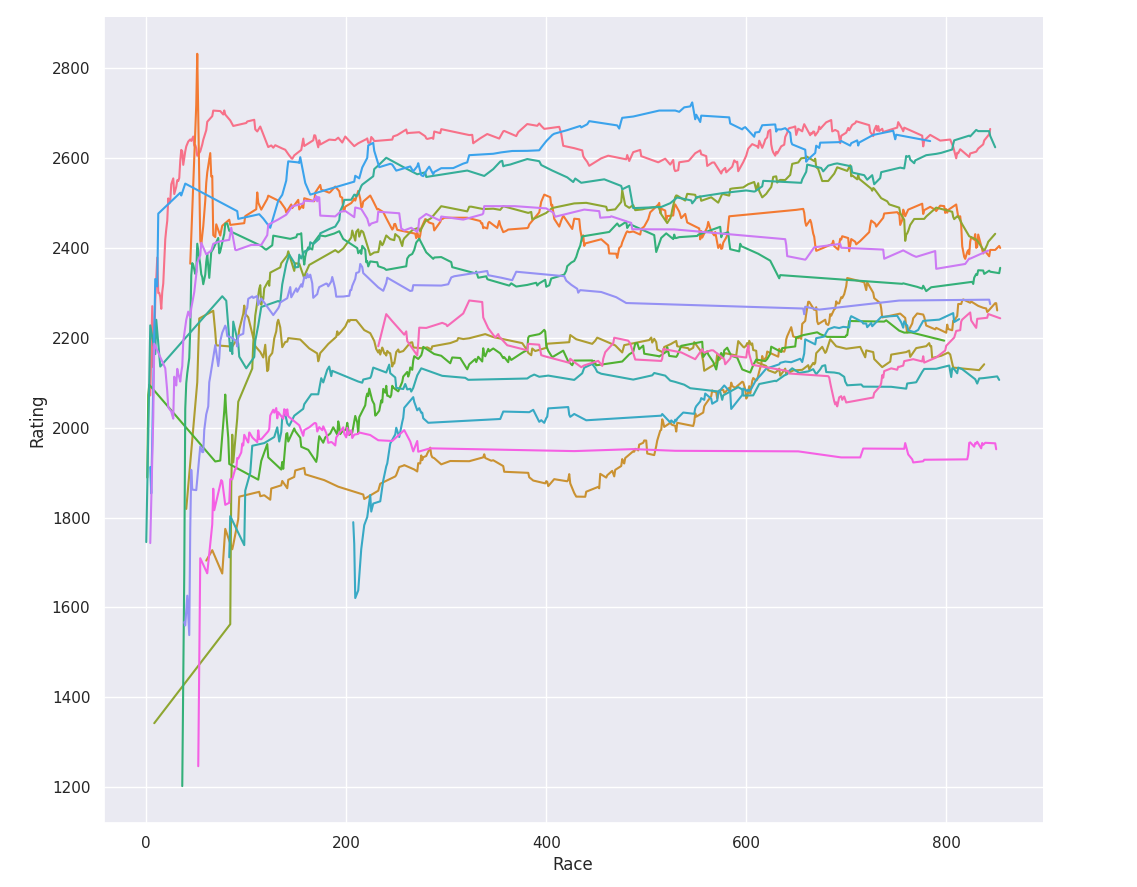
\includegraphics[width=0.75\linewidth]{figures/s1_trueskill_tuned.png}
	\caption{Super Metroid Map Rando season 1: TrueSkill ratings ($\mu - 2\sigma$), tuned settings}
	\label{fig:s1_trueskill_tuned}
	\end{figure}
	
	\subsection{Anchoring the rating scale}
	To try to improve the performance of the single-parameter models, we consider an issue that all these models share: when each player competes in their first race, their rating is initialized to a constant value. Because the games are zero-sum, the overall population of ratings remains centered around this value. This means that new players are initialized to a rating that is at the center of the skill distribution. Intuitively, this seems like an inappropriate choice of ``prior", because in practice it is more expected that new players would begin near the bottom of the skill distribution. There is also the practical problem that if new players are assigned an inaccurately high initial rating, they will likely experience declines in their ratings over the course of their first few games. Since players can interpret their rating as a reward for their performance, it can be demotivating for them to see their rating persistently go down from where it started. In the case of TrueSkill, this centered initialization is counteracted by the use of the lower confidence limit $\mu - 2\sigma$ in the ratings. However, in the case of the single-variable models, we do not have a $\sigma$ parameter available in order to construct such a confidence limit, so we must consider a different kind of solution.
	
	A related issue is that if the average skill level of players increases over time, this will not be reflected in the ratings, as the average rating remains locked to a constant. In this scenario, a consequence is that if a player takes a long break from playing and then returns, their rating value will now represent a higher level of skill than it did before, meaning that they are likely to experience a persistent decline in their rating. A returning player may assume their skills are rusty due to lack of practice, but again it may be demotivating if they find themselves unable to return to their previous rating level even after resharpening their skills.
	
	In the context of online multiplayer games, one mechanism to anchor the rating scale is to treat bots as a special type of player known to have unchanging ``skill" \cite{minka2018trueskill}. For the games that are played on \texttt{racetime.gg}, it is not necessarily feasible to create a bot that could successfully complete a game. As an alternative, instead of an bot, we can consider a ``dummy player" as participating in every race and getting a result tied for last place; we can then hold the dummy player's rating to a constant value (e.g. zero) as a way of anchoring the rating system as a whole. The initial rating $r_0$ for new players can then be set to some other value and becomes meaningful to tune as a hyperparameter.
	
	If we apply this to the Map Rando season 1 data, we see a substantial improvement to the model performance across all single-parameter model families:
	
	\begin{center}
	\begin{tabular}{l|l|l}
		Method & Hyperparameters & Kendall tau \\ \hline
		Pairwise Elo (sum) &  $r_0 = -1.6, \eta=0.07$ & 0.2251 \\
		Pairwise Elo (average) & $r_0 = -2.5, \eta=0.63$ & 0.2275 \\
		Exponential (Plackett-Luce) & $r_0 = -2.7, \eta=0.18$ & 0.2229 \\
		Gaussian (Thurstonian) & $r_0 = -1.3, \eta=0.11$ & 0.2234 \\
	\end{tabular}
	\end{center}
	
	Counterintuitively we found that the best performance resulted from using an initial rating substantially lower than the dummy player rating. With this initialization, when playing against an equal-rated opponent, a new player will tend to gain more points from a win than they lose from a loss, so with a mix of win/loss results they will tend to accumulate points just based on playing, even without empirical evidence of an improvement in skill. This can be interpreted as a sort of ``activity bonus" for new players, imitating the TrueSkill behavior discussed above. Again the improvement in model performance could be explained by new players being likely to improve rapidly in skill over the course of their first few games. 
	
	The ``dummy player" trick eliminates the zero-sum property of the rating system, as players will gain points from the dummy player while the dummy player will not lose any in return. This raises the possibility that over time the ratings may experience inflation as the overall amount of points in the system grows. There are a couple reasons to think this may not be a problem:
	\begin{itemize}
		\item  As a player's rating increases, the amount of points that they earn from winning against the dummy player decreases at least exponentially fast as a function of their rating (or even more rapidly, in the Gaussian case). This implies that in the absence of new players, at worst we can expect the long-term growth in total points to be bounded by a logarithmic function.
		\item  If new players enter the system, they will tend to counteract inflation in the ratings; e.g. if someone has a similar skill to a new player but has an artificially inflated rating, then they will be overrated compared to an actual new player who is assigned the (unchanging) initial score, and therefore they would be expected to lose points against them on average, which tends to contract the rating scale back down.

	\end{itemize}

	\subsection{Further improvements}
	There are a couple more improvements that we can apply to the single-parameter models:
	\begin{itemize}
		\item Instead of using a constant learning rate, we can apply a lower learning rate to higher-rated players. This technique has long been used in chess rating systems (USCF and FIDE). It is motivated by an assumption that higher-rated players tend to play more games and to have a slower rate of change in skill per game. In the chess rating systems, ratings are thresholded into 3 buckets, with a distinct learning rate applied for players within each bucket. We will apply a similar technique but instead use linear interpolation across given values $(\rho_1, \eta_1), (\rho_2, \eta_2), (\rho_3, \eta_3)$ so that the learning rate will vary continuously as a function of rating.
		\item Apply a rating floor, such that a player's rating will be clamped to this value instead of dropping below it. This can be seen as somewhat intuitive given the way that we have set up the dummy player to anchor the rating system at the bottom end: the ratings of new players are initialized to a value that represents being almost as bad as possible, so it does not make sense to allow them to drop far below that. And again, from the perspective of player experience, it could be demotivating to see one's rating drop seemingly without limit.
	\end{itemize}
	
	The use of a varying learning rate has some similarity to the use of uncertainty parameters $\sigma$ by TrueSkill; both have an effect of increasing the average size of rating updates for new players compared to experienced players. The key difference is that while TrueSkill learns a distinct uncertainty parameter for each player, for a single-parameter model we instead assume a deterministic relationship between rating level and uncertainty, with lower rating levels being associated with more uncertainty. In this way, the effect on the size of rating updates is based only on the player's current rating level, not on the number of games played or other aspects of the player's history.
	
	With these improvements, the gap in performance between TrueSkill and single-parameter models is narrowed significantly on the Map Rando season 1 data. We focus attention on the exponential and Gaussian models, setting aside the pairwise Elo models which we have seen perform relatively poorly. Player trajectories (top 15 most active players) are shown for the Plackett-Luce model in Figure \ref{fig:s1_plackett_luce}.
	\begin{center}
	\begin{tabular}{l|l|l}
		Method & Hyperparameters & Kendall tau \\ \hline
		Exponential (Plackett-Luce) & $\scriptstyle r_\text{initial}=0.25,\ r_\text{dummy}=1.35,\ \rho=[0, 1, 2],\ \eta=[0.6, 0.13, 0.09]$ & 0.2177 \\
		Gaussian (Thurstonian) & $\scriptstyle r_\text{initial}=0.3,\ r_\text{dummy}=0.9,\ \rho=[0, 1, 2],\ \eta=[0.65, 0.09, 0.07]$ & 0.2211 
	\end{tabular}
	\end{center}

	\begin{figure}
	\centering
	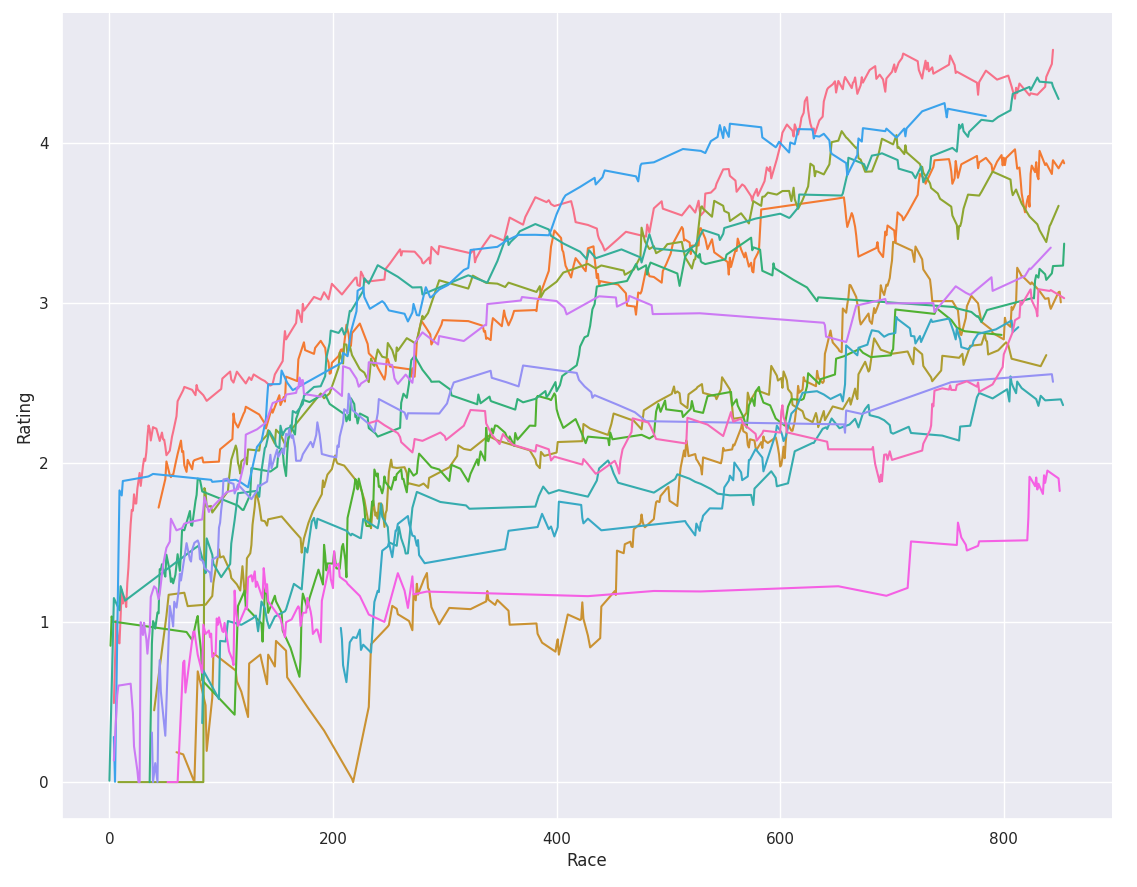
\includegraphics[width=0.75\linewidth]{figures/s1_plackett_luce.png}
	\caption{Super Metroid Map Rando season 1: Exponential (Plackett-Luce) ratings}
	\label{fig:s1_plackett_luce}
	\end{figure}
	
	We can then evaluate how these models perform going forward on Map Rando seasons~2 and~3 data. For this we keep the same hyperparameters tuned from the season 1 data, and apply it to the recorded races of seasons 2-3, with all ratings being freshly initialized, having no memory from season~1:
	\begin{center}
	\begin{tabular}{l|l|l}
		Method & Hyperparameters & Kendall tau \\ \hline
		Exponential (Plackett-Luce) & $\scriptstyle r_\text{initial}=0.25,\ r_\text{dummy}=1.35,\ \rho=[0, 1, 2],\ \eta=[0.6, 0.13, 0.09]$ & 0.1813 \\
		Gaussian (Thurstonian) & $\scriptstyle r_\text{initial}=0.3,\ r_\text{dummy}=0.9,\ \rho=[0, 1, 2],\ \eta=[0.65, 0.09, 0.07]$ & 0.1808 \\
		TrueSkill (default, $\mu$) &$\scriptstyle \sigma=8.33,\ \beta=4.17,\ \tau=0.083,\ \varepsilon=0.1$ & 0.1738 \\
		TrueSkill (tuned, $\mu - 2\sigma$) & $\scriptstyle \sigma=5.0,\ \beta=2.5,\ \tau=0.12,\ \varepsilon=0.001$ & \textbf{0.1732}
	\end{tabular}
	\end{center}

	\section{Conclusions}
	In the example data, we see that TrueSkill is providing superior predictive performance, while single-parameter models have certain advantages because of their simpler, more intuitive behavior. For example, the single-parameter models never cause an increase to a player's rating when they DNF; and rating updates in any given race are predictable based on the race outcome and the current ratings of the players, not dependent on their previous history or hidden parameters. So for a given application, a single-parameter model could be adopted based on these advantages, with the understanding that it likely comes with a trade-off in the ability of the model to accurately estimate players' skill level.
	
	One last observation is that across all 3 seasons of Map Rando race data, there are 176 instances of a player getting last place in a race while receiving a positive update to their score, and in every one of these instances the player was one of multiple players who DNF'd the race. This leads to a suspicion that this behavior is primarily a result of how TrueSkill handles ties, which as we argued above, does not seem reasonable when applied to race DNFs. Therefore, it is conceivable that this issue might be resolvable by handling DNFs in a different way.
	
	\printbibliography	
\end{document}